% arara: lualatex: {draft: yes}
% arara: makeindex: {style: gind}
% arara: lualatex: {draft: yes}
% arara: lualatex
% arara: clean: { files:[mydoc.ilg, mydoc.out, mydoc.gls, mydoc.ind, mydoc.aux, mydoc.idx, mydoc.log,mydoc.toc, mydoc.hd] }
\documentclass{ltxdoc}
\usepackage{mysty}
\def\myscript{ltximg}
\def\fileversion{v1.5}
\def\filedate{2017-12-21}
\def\rulecolor{\color{SlateBlue}}

% email https://tex.stackexchange.com/a/663
\catcode`\_=11\relax%
\newcommand\email[1]{\_email #1\q_nil}%
\def\_email#1@#2\q_nil{%
  \href{mailto:#1@#2}{{\emailfont #1\emailampersat #2}}%
}%
\newcommand\emailfont{\sffamily}%
\newcommand\emailampersat{{\color{blue}\footnotesize@}}%
\catcode`\_=8\relax% %  

% Table of contents, need change font style
\tocsetup{%
 title=Contents\quad{\rulecolor\leaders\vrule height3.4pt depth-3pt\hfill\null},
 title/after= \vspace{3pt},
 title/font= \sffamily\bfseries\Large,%
 title/top=10pt,%
 title/bottom=0pt,%
 twocolumns,
 section/skip=4pt plus2pt minus2pt,%
 subsection/skip=0pt plus2pt minus2pt,
 section/leaders,section/dotsep,%
 after=\vspace{-3pt}\noindent{\rulecolor\hrule height3.4pt depth-3pt\relax},
}

\begin{document}

\title{%
    \textffm{latex environments}\\[3pt]%
    \scalebox{3.4}{\LTXimg}\\[2pt]%
    \textls[150]{\textffm{to image format}}\\%
    \Large
    \fileversion{} --- \filedate\thanks{%
    This file describes a documentation for version \fileversion, last revised \filedate.}\\[25pt]%
    \author{%
    \large%
    \raisebox{-1pt}{\textcopyright}{}2013--2017 by Pablo González L%
    \thanks{E-mail:<\email{pablgonz@yahoo.com}>}%
    }%
\small
\textsc{ctan}: \url{http://www.ctan.org/pkg/ltximg}\\
\textsc{git}: \url{https://github.com/pablgonz/ltximg}
\vspace*{-2cm}
}%
\date{}
\maketitle

\begin{abstract}
\ltximg is a \prgname{perl} \emph{script} that automates the process of extracting and 
converting environments provided by \pkgname{tikz}, \pkgname{pstricks} and 
other packages from input file to image formats in individual files using \prgname{ghostscript} 
and \prgname{poppler-utils}. Generates a file with only extracted environments and another with environments 
converted to \ics{includegraphics}.
\end{abstract}

\tableofcontents
\setlength{\parskip}{3pt} 

\section{Motivation}
The original idea was to extend the functionality of the \scriptname{pst2pdf} 
script (only for \env{pspicture} and \env{postscript}) to work with \env{tikzpicture} 
and other environments. 

The \pkgname{tikz} package allows to externalize the environments, but, the idea was to be 
able to extend this to any type of environment covering three central points:

\begin{enumerate}[font=\small, noitemsep,leftmargin=*]
\item Generate separate files for environments and converted into images.
\item Generate a file with only the extracted environments.
\item Generate a file replacing the environments by \ics{includegraphics}.
\end{enumerate}

From the side of \TeX{} there are some packages that cover several of these 
points such as the \pkgname{preview}, \pkgname{xcomment}, \pkgname{external} and \pkgname{cachepic} packages among others, 
but none covered all points.

In the network there are some solutions in \texttt{bash} that were able to 
extract and convert environments, but in general they presented problems when the document 
contained \emph{verbatim style} code or were only available for \OSsystem{Linux}.

Analysed the situation the best thing was to create a new \emph{script} that was able 
to cover the three points and was multi platform, the union of all these ideas is 
born \ltximg. Finding the correct \emph{regular expressions} and writing \emph{documentation} 
would be the great mission (which does not end yet).

\thispagestyle{plain}
\newpage
\pagestyle{myheader}
\section{Required Software}
\label{sec:software}

For the complete operation of \ltximg{} you need to have a modern \hologo{TeX} 
distribution such as \hologo{TeX}Live 2017 or \hologo{MiKTeX} 2.9, have a version equal to or 
greater than \liningnums{5.22} of \prgname{perl}, a version equal to or greater than \liningnums{9.19} of 
\prgname{ghostscript} and have a version equal to or greater than \liningnums{0.52} of 
\textcolor{ForestGreen}{\ttfamily\bfseries poppler-utils}. 

The distribution of \hologo{TeX}Live 2017 for \OSsystem{Windows} includes \ltximg{} and all 
requirements, \hologo{MiKTeX} users must install the appropriate software for full operation.

The script has been tested on \OSsystem{Windows} (version 10) and \OSsystem{Linux} (fedora 27) in x64 architecture using 
\prgname{ghostscript} \liningnums{v9.20}, \textcolor{ForestGreen}{\ttfamily\bfseries poppler-utils} \liningnums{v0.52} to \liningnums{v0.60} and 
\prgname{perl} from \liningnums{v5.22} to \liningnums{v5.26}.

\section{How it works}
\label{sec:howtowork}
It is important to have a general idea of how the \emph{extraction and conversion} 
process works and the requirements that must be fulfilled so that everything 
works correctly, for this we must be clear about some concepts related to how to 
work with the \emph{verbatim content}, the  \emph{input file}, the \emph{output file} and the 
\emph{steps process}.

\subsection{The input file}
\label{sec:inputfile}
The \meta{input file} must comply with certain characteristics in
order to be processed, the content at the beginning and at the end of the \meta{input file} 
is treated in a special way, before \ics{documentclass} can only be commented lines and
after \lstinline|\end{document}| can go any type of content, the \emph{script} internally 
will split the \meta{input file} at this points.
 
If the \meta{input file} contains files using \ics{input} or \ics{include} these 
will not be processed, from the side of the \emph{script} they only represent 
lines within the file, if you want them to be processed it is better to use the 
\scriptname{latexpand} first and then process the file.

Like \ics{input} or \ics{include}, blank lines, vertical spaces and tab 
characters are treated literally, for the \emph{script} the \meta{input file} is just a set of 
characters, as if it was a simple text file. It is advisable to format the source code \meta{input file} 
using utilities such as lines such as \prgname{chktex} and \scriptname{latexindent}, especially if you want to 
extract the source code of the environments.

An example of the \meta{input file}:

\begin{examplecode}
% some commented lines at begin document
\documentclass{article}
\usepackage{tikz}
\begin{document}
Some text
\begin{tikzpicture}
Some code
\end{tikzpicture}
Always use \verb|\begin{tikzpicture}|
and \verb|\end{tikzpicture}| to open
and close environment
\begin{tikzpicture}
Some code
\end{tikzpicture}
Some text
\end{document}
% some lines after end document
\end{examplecode}

\subsection{Verbatim contents}
\label{sec:verbatim}

One of the greatest capabilities of \ltximg{} script is to skip the complications
that \emph{verbatim style} content produces with the extraction of environments. 
In order to skip the complications, the verbatim content is classified into
three types: 

\begin{itemize}
	\item Verbatim in line
	\item Verbatim standard
	\item Verbatim write
\end{itemize}

Each of these classifications works differently within the creation and 
extraction process using different regular expressions for it.
\newpage

\subsubsection{Verbatim in line}
\label{sec:verbatim:inline}
The small pieces of code written in the same line using a verbatim command are 
considered \meta{verbatim in line}, such as 
\texttt{\textbackslash verb\textbar\meta[type=tt]{code}\textbar}. The script 
supports most verbatim commands, the packages \pkgname{minted}, \pkgname{fancyvrb} and \pkgname{listings} have 
been tested and are fully  supported by \ltximg. The \emph{script} detects the verbatim command generates 
by \ics{newmint} and \ics{newmintinline} and the following command list:

\begin{multicols}{3}
\begin{itemize}[font=\sffamily\small, noitemsep,leftmargin=*]
\small
\item \ics{mint}
\item \ics{spverb}
\item \ics{qverb}
\item \ics{fverb}
\item \ics{verb}
\item \ics{Verb}
\item \ics{lstinline} 
\item \ics{pyginline}
\item \ics{pygment}
\item \ics{tcboxverb}
\item \ics{mintinline}
\end{itemize}
\end{multicols}

Some packages define abbreviated versions for verbatim commands as \ics{DefineShortVerb}, \ics{lstMakeShortInline}
and \ics{MakeSpecialShortVerb}, the \emph{script} detects commands if declared explicitly in \meta{input file}.

The following consideration should be kept in mind for some packages that use
abbreviations for verbatim commands, such as \pkgname{shortverb} or \pkgname{doc} 
for example in which there is no explicit command in the document by means of 
which the abbreviated form can be detected, for automatic detection need to find 
\ics{DefineShortVerb} explicitly to process it correctly. 
The solution is quite simple, just add in \meta{input file}:

\begin{examplecode}
\UndefineShortVerb{\|}
\DefineShortVerb{\|}
\end{examplecode}

depending on the package you are using. If your verbatim command is not supported 
by default or \ltximg{} can not detect, use the options described in \ref{sec:optline} and \ref{sec:optfile}.

\subsubsection{Verbatim standard}
\label{sec:verbatim:std}
These are the classic environments for writing code are considered \meta{verbatim standard}, 
such as \env{verbatim} and \env{lstlisting} environments. The following list is considered 
as \meta{verbatim standard} environments:

\begin{multicols}{4}
\begin{itemize}[font=\sffamily\small, noitemsep,leftmargin=*]
\sffamily\small
\item Example
\item CenterExample
\item SideBySideExample
\item PCenterExample
\item PSideBySideExample
\item verbatim
\item Verbatim
\item BVerbatim
\item LVerbatim
\item SaveVerbatim
\item PSTcode
\item LTXexample
\item tcblisting
\item spverbatim
\item minted
\item listing
\item lstlisting
\item alltt
\item comment
\item chklisting
\item verbatimtab
\item listingcont
\item boxedverbatim
\item demo
\item sourcecode
\item xcomment
\item pygmented
\item pyglist
\item program
\item programl
\item programL
\item programs
\item programf
\item programsc
\item programt
\end{itemize}
\end{multicols}

The \emph{script} detects \meta{verbatim standard} environments generates by commands:

\begin{multicols}{2}
\begin{itemize}[font=\sffamily\small, noitemsep,leftmargin=*]
\small
\item \ics{DefineVerbatimEnvironment}
\item \ics{NewListingEnvironment}
\item \ics{DeclareTCBListing}
\item \ics{ProvideTCBListing}
\item \ics{lstnewenvironment}
\item \ics{newtabverbatim}
\item \ics{specialcomment}
\item \ics{includecomment}
\item \ics{newtcblisting}
\item \ics{NewTCBListing}
\item \ics{newverbatim}
\item \ics{NewProgram}
\item \ics{newminted}
\end{itemize}
\end{multicols}

If any of the  \meta{verbatim standard} environments is not supported by default or the script can
not detected, you can use the options described in \ref{sec:optline} and \ref{sec:optfile}.

\subsubsection{Verbatim write}
\label{sec:verbatim:write}
Some environments have the ability to write external files directly, these environments are considered
\meta{verbatim write}, such as \env{filecontents} or \env{VerbatimOut} environments. The following list 
is considered as \meta{verbatim write} environments:

\begin{multicols}{3}
\begin{itemize}[font=\sffamily\small, noitemsep,leftmargin=*]
\small
\item filecontents
\item tcboutputlisting
\item tcbexternal
\item extcolorbox
\item extikzpicture
\item VerbatimOut
\item verbatimwrite
\item filecontentsdef
\item filecontentshere
\end{itemize}
\end{multicols}

The \emph{script} detects \meta{verbatim write} environments generates by commands:
\begin{multicols}{2}
\begin{itemize}[font=\sffamily\small, noitemsep,leftmargin=*]
\small
\item \ics{renewtcbexternalizetcolorbox}
\item \ics{renewtcbexternalizeenvironment}
\item \ics{newtcbexternalizeenvironment}
\item \ics{newtcbexternalizetcolorbox}
\end{itemize}
\end{multicols}

If any of the  \meta{verbatim write} environments is not supported by default or the script can
not detected, you can use the options described in \ref{sec:optline} and \ref{sec:optfile}.

\subsection{Steps process}
\label{sec:steps:process}
For creation of the image formats, extraction of code and creation of an 
output file, \ltximg{} need a various steps. Let's assume that the \meta{input file} is \sysfile{test.tex}, 
\meta{output file} is \sysfile{test-out}, the working directory are \sysdir{workdir}, the directory
for images are \sysdir{workdir/images} and the user's temporary directory is \sysdir{tmp} and we
want to generate images in \iext{pdf} format together with the source codes of the environments.

\begin{description}[font=\sffamily\small, leftmargin=0em,style=nextline]
\item[Comment and ignore] 
The first step is read and validated \oarg[type=rm,cf=gray,sbc=optcolor,ac=gray]{options} from the command 
line and \sysfile{test.tex}, verifying that \sysfile{test.tex}, \sysfile{test-out} and the 
directory \sysdir{images} are in \sysdir{workdir}, create the directory \sysdir{workdir/images} if it does 
not exist and a temporary directory \sysdir{tmp/hG45uVklv9}. The entire file \sysfile{test.tex} is loaded 
in memory and proceeds (in general terms) as follows:

\begin{quotation}
Search the words \lstinline|\begin{| and \lstinline|\end{| in verbatim standard, verbatim write, verbatim in line and 
commented lines, if it finds them, converts to \lstinline|\BEGIN{| and \lstinline|\END{|, then places all code to 
extract inside the \lstinline|\begin{preview}| \ldots \lstinline|\end{preview}|.
\end{quotation}

At this point all the code you want to extract is inside \lstinline|\begin{preview}| \ldots \lstinline|\end{preview}|
and the files \sysfile{test-fig-1.tex}, \sysfile{test-fig-2.tex}, \ldots{} are generated and saved in \sysdir{images}.

\item[Create random file] 
In the second step, with the file already loaded in memory, creating a temporary file with a 
random number (1981 for example) and proceed in two ways according to the \oarg[type=rm,cf=gray,sbc=optcolor,ac=gray]{options} 
passed to the script:

\begin{enumerate}
\item If script is call \emph{whitout} \cmdopt[n]{noprew} options, adds the
following lines to the beginning of the \sysfile{test.tex} (in memory):

\begin{examplecode}
\AtBeginDocument{%
\RequirePackage[active,tightpage]{preview}
\renewcommand\PreviewBbAdjust{-60pt -60pt 60pt 60pt}}%
% rest of input file
\end{examplecode}
And save in a temporary file \sysfile{test-fig-1981.tex} in \sysdir{workdir}.

\item If script is call \emph{whit} \cmdopt[n]{noprew} options, all code to extract
its put inside the \env{preview} environment. The \lstinline|\begin{preview}|\ldots \lstinline|\end{preview}| 
lines are only used as delimiters for extracting the content \emph{without} using the package \pkgname{preview}.

Creating a temporary file \sysfile{test-fig-1981.tex} in \sysdir{workdir}  
whit the same preamble of \sysfile{test.tex} but the body only contains code that you want to extract.
\end{enumerate}

\item[Generate image formats] 
In the third step the script run \meta[type=tt,cf=ForestGreen,ac=ForestGreen]{compiler}
\prgopt*{recorder} \prgopt*{shell-escape} \sysfile{test-fig-1981.tex} generating the file
\sysfile{test-fig-1981.pdf} whit all code extracted, move \sysfile{test-fig-1981.pdf} 
to \sysdir{tmp/hG45uVklv9}, separate in individual files \sysfile{test-fig-1.pdf}, \sysfile{test-fig-2.pdf}, \ldots{}   
and copy to \sysdir{workdir/images/}. The file \sysfile{test-fig-1981.tex} is moved to the \sysdir{workdir/images/} 
and rename to \sysfile{test-fig-all.tex}.

Note the options passed to \meta[type=tt,cf=ForestGreen,ac=ForestGreen]{compiler} does not include \prgopt*{output-directory} 
(it is not supported) and always use \prgopt*{recorder} \prgopt*{shell-escape} you must keep this in mind if you use \prgname{arara}.

\item[Create output file] 
In the fourth step the script creates the output file \sysfile{test-out.tex} converting all extracted code to 
\ics{includegraphics} and adding the following lines at end of preamble:

\begin{examplecode}
\usepackage{graphicx}
\graphicspath{{images/}}
\usepackage{grfext}
\PrependGraphicsExtensions*{.pdf}
\end{examplecode}

If the packages \pkgname{graphicx} and \pkgname{grfext} are already loaded and the command \ics{graphicspath} 
is found in the input file were detected automatically and only the changes will be added then proceed to
run \meta[type=tt,cf=ForestGreen,ac=ForestGreen]{compiler} \prgopt*{recorder} \prgopt*{shell-escape} \sysfile{test-out.tex} 
generating the file \sysfile{test-out.pdf}.
\end{description}
Now the script read the files \sysfile{test-fig-1981.fls} and \sysfile{test-out.fls}, extract the information from the 
temporary files generated in the process and then delete them together with the directory \sysdir{tmp/hG45uVklv9}.
An example for input and output file:

\begin{minipage}[c]{0.5\textwidth}
\begin{examplecode}
\documentclass{article}
\usepackage{tikz}
\begin{document}
Some text
\begin{tikzpicture}
Some code
\end{tikzpicture}
Always use \verb|\begin{tikzpicture}|
and \verb|\end{tikzpicture}| to open 
and close environment
\begin{tikzpicture}
some code
\end{tikzpicture}
Some text
\end{document}
\end{examplecode}
\begin{flushleft}
\sysfile{test.tex}
\end{flushleft}
\end{minipage}
\begin{minipage}[c]{0.5\textwidth}
\begin{examplecode}
\documentclass{article}
\usepackage{tikz}
\usepackage{graphicx}
\graphicspath{{images/}}
\usepackage{grfext}
\PrependGraphicsExtensions*{.pdf}
\begin{document}
Some text
\includegraphics[scale=1]{test-fig-1}
Always use \verb|\begin{tikzpicture}|
and \verb|\end{tikzpicture}| to open 
and close environment
\includegraphics[scale=1]{test-fig-2}
Some text
\end{document}
\end{examplecode}
\begin{flushleft}
\sysfile{test-out.tex}
\end{flushleft}
\end{minipage}
\newpage

\section{Extract content}
\label{sec:extract}
The script provides two ways to extract content from a \hologo{LaTeX} file, using \meta[type=rm,cf=optcolor,ac=gray]{environments} 
and \meta[type=rm,cf=optcolor,ac=gray]{docstrip} tags. Some environment (including a starred \texttt{\small\bfseries\textcolor{red}{*}} version) are suported by default and if the environments are nested, the outermost will be extracted.

\subsection{Default environments}
\label{sec:extract:env}
\DescribeTE{preview}
Environment provide by \pkgname{preview} package. If \env{preview} environments
found in the input file will be extracted and converted these. Internally
converts all environments to extract in \env{preview} environments.
Is better comment this package in preamble unless the option \cmdopt[n]{noprew}{} is
used.

\vspace{\baselineskip}

\DescribeTE{pspicture}
Environment provide by \pkgname{pstricks} package. The plain
syntax \lstinline|\pspicture ... \endpspicture| its converted to
\lstinline|\begin{pspicture} ... \end{pspicture}|.
\vspace{\baselineskip}

\DescribeTE{psgraph}
Environment provide by \pkgname{pst-plot} package. The plain syntax \lstinline|\psgraph ... \endpsgraph|
its converted to \lstinline|\begin{psgraph} ... \end{psgraph}|.

\vspace{\baselineskip}

\DescribeTE{postscript}
Environment provide by \pkgname{pst-pdf} and \pkgname{auto-pst-pdf} packages.
Since the \pkgname{pst-pdf} and \pkgname{auto-pst-pdf} packages internally use
the \pkgname{preview} package, is better comment this in preamble.

\vspace{\baselineskip}

\DescribeTE{tikzpicture}
Environment provide by \pkgname{tikz} package. The plain syntax \lstinline|\tikzpicture ... \tikzpicture|
its converted to \lstinline|\begin{tikzpicture} ... \end{tikzpicture}|
but no a short \lstinline|\tikz...;|.
\vspace{\baselineskip}

\DescribeTE{pgfpicture}
Environment provide by \pkgname{pgf} package. Since the script uses a
\emph{recursive regular expression} to extract environments, no presents problems
if present \lstinline|pgfinterruptpicture|.
\vspace{\baselineskip}

\DescribeTE{PSTexample}
Environment provide by \pkgname{pst-exa} packages. The script automatically detects the 
\lstinline|\begin{PSTexample}|  \lstinline|...\end{PSTexample}| 
environments and processes them as separately compiled files. The user should have loaded the
package with the [\pkgopt{swpl}] or [\pkgopt{tcb}] option and run the script
using \cmdopt{latex}{} or \cmdopt{xetex}.

If you need to extract more environments you can use one of the options described in \ref{sec:optline} or \ref{sec:optfile}.
\subsection{Extract whit docstrip tags}
\label{sec:extract:tag}
\DescribeTE*{ltximg}
All content included between \lstinline|%<*ltximg> ... %</ltximg>| is extracted. 
The tags can not be nested and should be at the beginning of the line and in separate lines.

\begin{examplecode}
% no space before open tag %<* 
%<*ltximg>
code to extract 
%</ltximg>
% no space before close tag %</ 
\end{examplecode}

\subsection{Prevent extraction and remove}
\label{sec:noextract}
Sometimes you do not want to extract all the environments from the input file or you want to 
remove environments or arbitrary content, for example auxiliary files to generate a graphic. 
The script provides a convenient way to solve this situation.

\DescribeTE{nopreview}
Environment provide by \pkgname{preview} package. Internally the script
converts all no extract environments to \lstinline|\begin{nopreview} ... \end{nopreview}|.
Is better comment this package in preamble unless the option \cmdopt[n]{noprew}{} is used.
\vspace{\baselineskip}

\DescribeTE*{noltximg}
All content betwen \lstinline|%<*noltximg> ... %</noltximg>| are ignored and no
extract. The start and closing of the tag must be at the beginning of the line.

\begin{examplecode}
% no space before open tag %<* 
%<*noltximg>
no extract this
%</noltximg>
% no space before close tag %</ 
\end{examplecode}

\DescribeTE*{remove}
All content betwen \lstinline|%<*remove> ... %</remove>| are deleted in the output file. The start and closing
of the tag must be at the beginning of the line.

\begin{examplecode}
% no space before open tag %<* 
%<*remove>
lines removed in output file
%</remove>
% no space before close tag %</ 
\end{examplecode}

If you want to remove specific environments automatically you can use one of the options described in \ref{sec:optline} or \ref{sec:optfile}.
\section{Image Formats}
\label{sec:image:format}
The image formats generated by the script are the following:

\DescribeIF{pdf}
The image format generated using \prgname{ghostscript}. The line executed by the system is:

\begin{examplecmd}
[user@machine ~:]§ gs -q -dNOSAFER -sDEVICE=pdfwrite -dPDFSETTINGS=/prepress
\end{examplecmd}

\DescribeIF{eps}
The image format generated using \prgname{pdftoeps}. The line executed by the system is:

\begin{examplecmd}
[user@machine ~:]§ pdftops -q -eps
\end{examplecmd}

\DescribeIF{png}
The image format generated using \prgname{ghostscript}. The line executed by the system is:

\begin{examplecmd}
[user@machine ~:]§ gs -q -dNOSAFER -sDEVICE=pngalpha -r 150
\end{examplecmd}

\DescribeIF{jpg}
The image format generated using \prgname{ghostscript}. The line executed by the system is:
\begin{examplecmd}
[user@machine ~:]§ gs -q -dNOSAFER -sDEVICE=jpeg -r 150 -dJPEGQ=100 \
                      -dGraphicsAlphaBits=4 -dTextAlphaBits=4
\end{examplecmd}

\DescribeIF{ppm}
The image format generated using \prgname{pdftoppm}. The line executed by the system is:

\begin{examplecmd}
[user@machine ~:]§ pdftoppm -q -r 150
\end{examplecmd}

\DescribeIF{tif}
The image format generated using \prgname{ghostscript}. The line executed by the system is:

\begin{examplecmd}
[user@machine ~:]§ gs -q -dNOSAFER -sDEVICE=tiff32nc -r 150
\end{examplecmd}

\DescribeIF{svg}
The image format generated using \prgname{pdftocairo}. The line executed by the system is:

\begin{examplecmd}
[user@machine ~:]§ pdftocairo -q -r 150
\end{examplecmd}

\DescribeIF{bmp}
The image format generated using \prgname{ghostscript}. The line executed by the system is:

\begin{examplecmd}
[user@machine ~:]§ gs -q -dNOSAFER -sDEVICE=bmp32b -r 150
\end{examplecmd}
\newpage

\section{How to use}
\subsection{Syntax}
The syntax for \ltximg{} is simple:

\begin{examplecmd}
[user@machine ~:]§ ltximg `\small\meta[type=tt,cf=ForestGreen,ac=ForestGreen]{compiler} \oarg[type=tt,cf=gray,sbc=optcolor,ac=gray]{options} \textcolor{gray}{\texttt{[-\/-]}} \meta[type=tt,cf=OrangeRed,ac=OrangeRed]{file.ext}`
\end{examplecmd}

The extension \meta[type=tt,cf=OrangeRed,ac=OrangeRed]{ext} for \meta{input file} are \fext{tex} or \fext{ltx}, 
relative or absolute paths for files and directories is not supported. If used without \meta[type=tt,cf=ForestGreen,ac=ForestGreen]{compiler} 
and \oarg[type=tt,cf=gray,sbc=optcolor,ac=gray]{options} the extracted environments are converted to \iext{pdf} 
image format and saved in the \sysdir{images} directory using \prgname*{pdflatex} and \pkgname{preview} package.

\subsection{Options in command line}
\label{sec:optline}
\ltximg{} provides a \emph{command line interface} with short and long option names. 
They may be given before the name of the file. Also, the order of specifying the 
options is significant. Certain options accept a list separate by commas, this require a separated by 
white space or equals sign \textcolor{red}{\texttt{=}} between option and list and if it's the last option 
need \textcolor{red}{\texttt{-\/-}} at the end. Multiple short options can be bundling.

\DescribeCmd[h]{help}{bolean}{off}
Display a command line help text and exit.

\DescribeCmd[l]{license}{bolean}{off}
Display a license text and exit.

\DescribeCmd[v]{version}{bolean}{off}
Display the current version (1.5) and exit.

\DescribeCmd[d]{dpi}{int}{150}
Dots per inch for images files.

\DescribeCmd[t]{tif}{bolean}{off}
Create a .\iext{tif} images files using \prgname{ghostscript}. 

\DescribeCmd[b]{bmp}{bolean}{off}
Create a .\iext{bmp} images files using \prgname{ghostscript}. 

\DescribeCmd[j]{jpg}{bolean}{off}
Create a .\iext{jpg} images files using \prgname{ghostscript}. 

\DescribeCmd[p]{png}{bolean}{off}
Create a .\iext{png} transparent image files using \prgname{ghostscript}.

\DescribeCmd[e]{eps}{bolean}{off}
Create a .\iext{eps} image files using \prgname{pdftops}.

\DescribeCmd[s]{svg}{bolean}{off}
Create a .\iext{svg} image files using \prgname{pdftocairo}.

\DescribeCmd[P]{ppm}{bolean}{off}
Create a .\iext{ppm} image files using \prgname{pdftoppm}. 

\DescribeCmd[g]{gray}{bolean}{off}
Create a gray scale for all images using \prgname{ghostscript}. The line before this options is:

\begin{examplecmd}
[user@machine ~:]§ gs -q -dNOSAFER -sDEVICE=pdfwrite -dPDFSETTINGS=/prepress        \
                      -sColorConversionStrategy=Gray -dProcessColorModel=/DeviceGray
\end{examplecmd}

\DescribeCmd[f]{force}{bolean}{off}
Try to capture \lstinline|\psset{...}| and \lstinline|\tikzset{...}| to extract.

\DescribeCmd[n]{noprew}{bolean}{off}
Create images files without \pkgname{preview} package.

\DescribeCmd[m]{margin}{numeric}{0}
Set margins in bp for \scriptname{pdfcrop}.

\DescribeCmd[o]{output}{string}{empty}
Create output file whit all environments converted in image. The output file name must not contain extension.

\DescribeCmd{imgdir}{string}{/images}
The folder for save images and source code.

\DescribeCmd{verbose}{bolean}{off}
Show verbose information in screen and change \prgopt*{interaction} for compiler.

\DescribeCmd{srcenv}{bolean}{off}
Create separate files whit only code for all environment.

\DescribeCmd{srcenv}{bolean}{off}
Create sub files whit preamble and code for all environment.

\DescribeCmd{arara}{bolean}{off}
Use \prgname{arara} for compiler files, need to pass \prgopt*{recorder} option to input file\par
\lstinline|% arara : <compiler> : {options: "-recorder"}|

\DescribeCmd{xetex}{bolean}{off}
Using \prgname*{xelatex} compiler for create images.

\DescribeCmd{latex}{bolean}{off}
Using \prgname*{latex}\texttt{\bfseries\guillemotright}\prgname*{dvips}\texttt{\bfseries\guillemotright}\prgname*{ps2pdf} compiler in input file to create images
and \prgname*{pdflatex} for output file.

\DescribeCmd{dvips}{bolean}{off}
Using \prgname*{latex}\texttt{\bfseries\guillemotright}\prgname*{dvips}\texttt{\bfseries\guillemotright}\prgname*{ps2pdf} for compiler input and output file.

\DescribeCmd{dvipdf}{bolean}{off}
Using \prgname*{latex}\texttt{\bfseries\guillemotright}\prgname*{dvipdfmx} process for create images.

\DescribeCmd{luatex}{bolean}{off}
Using \prgname*{lualatex} to compiler files.

\DescribeCmd{prefix}{string}{fig}
Add prefix append to each file created.

\DescribeCmd{norun}{bolean}{off}
Run script, but no create images.

\DescribeCmd{nopdf}{bolean}{off}
Don't create a .\iext{pdf} image files.

\DescribeCmd{nocrop}{bolean}{off}
Don't run \scriptname{pdfcrop} in image files.

\DescribeCmd{myverb}{string}{myverb}
Set custom verbatim command \lstinline+\verbcmd|<code>|+.

\DescribeCmd{clean}{doc\textbar pst\textbar tkz\textbar all\textbar off}{doc}
Removes specific text in output file.

\DescribeCmd{extrenv}{list separate by comma}{empty}
List of other environments to extract, need \texttt{-\/-} at end.\par

\DescribeCmd{skipenv}{list separate by comma}{empty}

List of environments that should not be extracted and that the script supports
by default, need \texttt{-\/-} at end.\par

\DescribeCmd{verbenv}{list separate by comma}{empty}

Add new verbatim environment support, need \texttt{-\/-} at end.\par

\DescribeCmd{writenv}{list separate by comma}{empty}

Add new verbatim write environment support, need \texttt{-\/-} at end.\par

\DescribeCmd{deltenv}{list separate by comma}{empty}
Delete environment in output file,  need -\/- at end. The deletion process only occurs 
if an output file is defined. It runs after having extracted and created the images 
completely and only affects the output file. For example, if the input file is something like this:

\subsection{Options in input file}
\label{sec:optfile}

Many of the ideas in this section are inspired by the \prgname{arara} program (I adore it).
A very useful way to pass options to the script is to place them in commented
lines at the beginning of the file, very much in the style of \prgname{arara}.

\DescribeOptFile*{\meta[ac=gray,cf=gray]{argument}}{option one, option two, option three, \ldots}
\DescribeOptFile*{\meta[ac=gray,cf=gray]{argument}}{option one, option two, option three, \ldots}[!]

The vast majority of the options can be passed into the input file. These should be put at
the beginning of the file in commented lines. If you are going to create
an output file and you do not want these lines to remain, it is better to
place them inside the \lstinline|%<*remove> ... %</remove>|. Like this:

\begin{examplecode}
%<*remove>
% ltximg : options : {png,srcenv,xetex}
% ltximg : extrenv : {description}
%</remove>
\documentclass{article}
\begin{document}
    some content
\end{document}
\end{examplecode}

\DescribeOptFile{options}{option one = value, option two = value, option three = value, \ldots}
This line is to indicate to the script which options need to process.

\DescribeOptFile{extrenv}{environment one, environment two, environment three, \ldots}
This line is to indicate to the script which environments, not supported by
default, are extracted.

\DescribeOptFile{skipenv}{environment one, environment two, environment three, \ldots}
This line is to indicate to the script which environments, of the ones
supported by default, should not be extracted.

\DescribeOptFile{verbenv}{verbatim environment one, verbatim environment two, \ldots}
This line is to indicate to the script which environments, its considerate a verbatim standard.

\DescribeOptFile{writenv}{verbatim environment write one, verbatim environment write two, \ldots}
This line is to indicate to the script which environments its consider verbatim write.

\DescribeOptFile{deltenv}{environment one, environment two, environment three, \ldots}
This line is to indicate to the script which environments are deleted.

\begin{examplecode}
% file-in.tex
% ltximg : options : {png,srcenv}
% ltximg : deltenv : {enumerate}
\documentclass[10pt]{article}
\begin{document}
    some content
\end{document}
\end{examplecode}
and the following line is used:
\begin{examplecmd}
[user@machine~:]§ ltximg -o file-out file-in.tex
\end{examplecmd}
\newpage

\section{Change history}%
\label{sec:change:history}
Some of the notable changes in the history of the \ltximg{} along with the 
versions, both development (devp) and public (ctan).

\setlist[itemize, 1]{label=\textendash,wide=0.5em, leftmargin=10pt}
% length for change history
\newlength\descrwidth
\settowidth{\descrwidth}{\textsf{v1.4.5, (ctan), 2013-01-23}}
\begin{description}[font=\small\sffamily, wide=0pt, style=multiline, leftmargin=\descrwidth]
\item [v1.5 (ctan), 2017-12-20]
    \begin{itemize} 
        \item Use GitHub to control version
        \item Rewrite and optimize most part of code and options
        \item Change pdf2svg for pdftocairo
        \item Complete support for pst-exa pack
        \item Escape characters in regex according to v5.4x.x
    \end{itemize}
\item [v1.4 (devp), 2016-11-29]
    \begin{itemize} 
        \item Remove and rewrite code for regex and system call
        \item Append arara compiler, clean and comment code
        \item Append dvips and dvipdfm for creation images
        \item Append bmp, tif image format
    \end{itemize}
\item [v1.3 (devp), 2016-08-14]
    \begin{itemize} 
        \item Rewrite some part of code , norun, nocrop, clean
        \item Suport minted and tcolorbox package for verbatim
        \item Escape some characters in regex according to v5.2x.x
        \item All options its read from command line and input file
        \item Use /tmp dir for work process
    \end{itemize}
\item [v1.2 (ctan), 2015-04-22]
    \begin{itemize} 
        \item Remove unused modules
        \item Add more image format
        \item Fix regex
    \end{itemize}
\item [v1.1 (ctan), 2015-04-21] 
    \begin{itemize}
        \item Change mogrify to gs for image formats
        \item Create output file
        \item Rewrite source code and fix regex
        \item Change format date to iso format
    \end{itemize}
\item [v1.0 (ctan), 2013-12-01] 
    \begin{itemize}
        \item First public release
    \end{itemize}
\end{description}

\newpage
\PrintIndex
\end{document}





For example, if the \pkgname{preview} package or \ics{tikzexternalize} 
is used, the following example will fail to be compiled:

\begin{examplecode}
\documentclass{article}
\usepackage{tikz}
\begin{document}
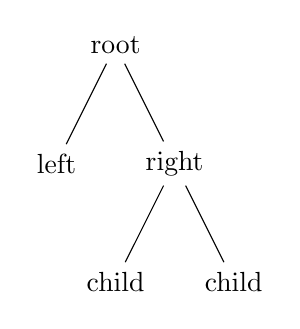
\begin{tikzpicture}
\node {root}
    child {node {left}}
    child {node {right}
    child {node {child}}
    child {node {child}}
    };
\end{tikzpicture}
Allway use \verb|\begin{tikzpicture}| and
\verb|\end{tikzpicture}| to open and close
\end{document}
\end{examplecode}

For example:

\begin{examplecmd}
[user@machine ~:]§ ltximg -e -p -j --srcenv --imgdir pics -o test-out test-in.ltx
\end{examplecmd}
or
\begin{examplecmd}
[user@machine ~:]§ ltximg -epj --srcenv --imgdir=pics -o test-out  test-in.ltx
\end{examplecmd}
produce a file \marg{test-out.ltx} with all environments extracted converted to \ics{includegraphics} and create
\sysdir{pics} dir whit all images format (\iext{pdf}, \iext{eps}, \iext{png}, \iext{jpg})
and source code in separate files using \prgname{pdlt} (pdf)LaTeX whit \pkgname{preview} package.

\begin{minipage}[c]{0.5\textwidht}
\begin{examplecode}
\documentclass{article}
\usepackage{tikz}
\begin{document}
Some text
\begin{tikzpicture}
Some code
\end{tikzpicture}
Allway use \verb|\begin{tikzpicture}| and
\verb|\end{tikzpicture}| to open and close
\begin{tikzpicture}
some code
\end{tikzpicture}
Some text
\end{document}
\end{examplecode}
\end{minipage}
\begin{minipage}[c]{0.5\textwidht}
...
\end{minipage}

If the last \oarg[type=tt,cf=gray,sbc=optcolor,ac=gray]{option} take a \emph{list separated by commas} you need \texttt{\bfseries\textcolor{optcolor}{-\/-}} at the end. 
